% \documentclass[11pt,a4paper,twocolumn,titlepage]{article}
\documentclass[11pt,a4paper,titlepage]{article}
\usepackage[margin=1in]{geometry}
\usepackage{amsmath}
\usepackage{amsthm}
\usepackage{amssymb}
\usepackage{graphicx}
\usepackage[pdftex]{hyperref}

\setlength{\parskip}{1em}


\title{CS 6230 Project Report\\\textbf{Parallel Computation of Betweenness Centrality}}
\author{Rui Dai, Sam Olds}
\date{\today}


\begin{document}
\maketitle
\newpage


% Outline:
% 1.) Introduction
%     * What is centrality
%     * Different types
%       * Degree
%       * Closeness
%       * Betweenness
%       * Page Rank!
%       * Many More: Eigenvector centrality, Katz centrality, Percolation
%         centrality, Cross-clique centrality, Freeman Centralization
%     * Why is it important
%     * What problems does it solve
%     * How is it used
%     * The type of centrality we focused on was betweenness centrality - it's
%       a lot of shortest path calculations.
% 2.) Related work
%     * How have other people already approached this problem
%     * The best known algorithms for different types of centrality
%     * Algorithms we looked at
%     * Floyd-Warshall $O(V^3)$
%     * Brandes $O(VE)$
% 3.) Implementation
%     * Challenges of implementing this in parallel
%     * Challenges of finding a validly large social graph
%     * Started with an adjacency matrix and matrix multiplication
%     * Moved onto brandes algorithm using an adjacency list
%       \cite{brandes2001faster}
%     * Finally, implemented a parallelized version of brandes found here
%       \cite{bader2006parallel}
% 4.) Experimentation
%     * Began with synthetic graphs. generated graphs this way
%     * Moved to facebook graph with 4000 vertices \cite{leskovec2012learning}
%     * Ended with a gplus graph with 107000 vertices
%       \cite{leskovec2012learning}
% 5.) Results
%     * Challenges of rendering large graphs
%     * Challenges of validating centrality
%     * Graphs of strong and weak scalability.
%     * Graphs of centrality found
% 6.) Conclusion
%     * MPI and OpenMP really sped up the processing time
% 7.) Future work
%     * We could continue working to improve the running time and finding more
%       graphs to run it on
%     * We used a shared memory model, it would be interesting to try and break
%       up the graph into a distributed memory model.



%% ============================= Introduction ============================= %%
\section{Introduction} % 1. introduction and motivation
\label{sec:intro}
%     * What is centrality
%     * Different types
%       * Degree
%       * Closeness
%       * Betweenness
%       * Page Rank!
%       * Many More: Eigenvector centrality, Katz centrality, Percolation
%         centrality, Cross-clique centrality, Freeman Centralization
%     * Why is it important
%     * What problems does it solve
%     * How is it used
%     * The type of centrality we focused on was betweenness centrality - it's
%       a lot of shortest path calculations.

In graph theory, centrality indicates the importance of a vertex in the
network. This concept is naturally applied on social network analysis. Imagine
you are producing a new product and want to find beta users. It's simple to let
users with high centrality to use and spread the news to their reachable
networks.

There are many different definitions of centrality, eg. degree centrality,
closeness centrality and betweenness centrality. In our project, we will use
the vertex betweenness centrality.

Betweenness centrality quantifies the number of times a node acts as a bridge
along the shortest path between two other nodes. It's not hard to imagine that
the computation of centrality is very expensive with all the operations with
shortest paths. Our goal of this project is parallel such computation and
leverage the technology of MPI/OPENMP we learned in class.

We will explain two algorithms we use for parallel centrality computation, with
experiments result and analysis. 



%% ============================= Related Work ============================= %%
\section{Related Work} % 2. related work
\label{sec:related-work}
%     * How have other people already approached this problem
%     * The best known algorithms for different types of centrality
%     * Algorithms we looked at
%     * Floyd-Warshall $O(V^3)$
%     * Brandes $O(VE)$

Centrality was first introduced as a measure for quantifying the control of a
human on the communication between other humans in a social network by Linton
Freeman\cite{burt2009structural} In his conception. Ever since, the concept has
drawn many interests in cross-indiscipline area like network analysis and
social science.

Betweenness centralities in a graph involve calculating the shortest paths
between all pairs of vertices on a graph, which requires $\Theta(V^3)$ time
with the Floyd–Warshall\cite{Cormen:2001:IA:580470} algorithm. On sparse
graphs, Johnson's\cite{johnson1977efficient} algorithm may be more efficient,
taking $O(V^2 \log V + V E)$ time. In the case of unweighted graphs the
calculations can be done with Brandes' algorithm\cite{brandes2001faster} which
takes $\Theta(VE)$ time. Normally, these algorithms assume that graphs are
undirected and connected with the allowance of loops and multiple edges. When
specifically dealing with network graphs, often graphs are without loops or
multiple edges to maintain simple relationships (where edges represent
connections between two people or vertices). In this case, using Brandes'
algorithm will divide final centrality scores by 2 to account for each shortest
path being counted twice.

Breadth first search is also a great part in centrality computation as for the
shortest path part. Parallel BFS algorithms attracts many researchers to
explore, among those, \cite{beamer2013direction} proposed a two-direction way
to do BFS. [Sam will add more details]



%% ============================= Data ============================= %%
\section{Implementation} % 3. methods/algorithms
\label{sec:data}
%     * Challenges of implementing this in parallel
%     * Challenges of finding a validly large social graph
%     * Started with an adjacency matrix and matrix multiplication
%     * Moved onto brandes algorithm using an adjacency list
%       \cite{brandes2001faster}
%     * Finally, implemented a parallelized version of brandes found here
%       \cite{bader2006parallel}

We implemented our algorithms in C++ using OpenMP and MPI. Our final submission
employs an adjacency list to represent the graph and uses a parallel version
of the Brandes algorithm for calculating betweenness centrality. We will
examine the results more closely later, but it appears that this implementation
does not scale well which is most likely due to the fact that the graph is in
shared memory. Distributing the graph was a large hurdle we tried to avoid.


\subsection{Challenges}

The largest challenge was handling a graph distributed across processors.
Trying to partition the graph evenly among the workers could be a project on
its own. We encountered this problem when breaking up the adjacency matrix
among processors. We realized each processor might not have all of the edges
attached to each vertex in memory, which would complicate things. This was
solved simply by putting the whole graph in shared memory. However, it is
believed that this was the cause of the poor scaling performance.

The next challenge that arose was getting the graph data. During initial
development, a synthetic graph was used by looping through every vertex for
each vertex and creating and edge between them with a 25\% probability. Once we
were comfortable with our implementation we found a graph of Facebook friend
circles used in a Stanford paper \cite{leskovec2012learning} with 4039 vertices
and 88234 edges. We then found an even larger dataset of Google+ users used in
the same paper. This graph has 107614 vertices and 13673453 edges.

Validating the results was another challenge. We spent a fair number of hours
finding a way to visually render the graphs. The Graphviz open source project
was used, but was somewhat buggy. Ultimately, our validation of the metrics
became a visual inspection of the rendered graphs, which is less than ideal.
However, the nodes that were marked with higher centrality seemed to be the
correct ones.


\subsection{Graph Representation}

At first, the underlying representation we used was a sparse adjacency matrix.
We thought that this would allow for easier parallelization when performing the
matrix multiplication. However, it presented a few challenges during
implementation. First, an $n \times n$ matrix becomes memory demanding, even
thought most of the values are simply $0$. Second, we used the vertex ids as
the indices into the $n^2$ array, which didn't work for the Google+ dataset.
This dataset used $21$ digit long values, which means a separate data structure
would have been needed to map the vertex ids back to the matrix indices.

Instead, we switched to using an adjacency list to decrease the memory
footprint and simplify the vertex id handling. This had a few additional
advantages. With an adjacency list, we could easily figure out the total number
of vertices that exist in the graph by just getting the size of the list. This
also made it easy to split work among processors by making each processor
handle some chunk of the list. This made implementing the Brandes algorithm
more straightforward as this was the underlying graph representation used in
that paper.


\subsection{Algorithms}

Effectively, we implemented two different parallel algorithms for calculating
the betweenness centrality of a graph. As we mentioned in the introduction
section, vertex betweenness centrality is formally defined as:

\[ g(v) = \sum_{s \neq v \neq t}{\frac{\sigma_{st}(v)}{\sigma_{st}}} \]

\subsubsection{Matrix Multiplication}

Calculating betweenness centrality can be naively accomplished by calculating
the shortest path from every vertex to every other vertex. This was our initial
approach. We used a breadth first search technique using matrix multiplication
because it was believed that this would make it easy to parallelize. Using
matrix multiplication to find the shortest paths behaves as follows:

For our $n \times n$ matrix, we initialize a vector of size $n$ to all $0$s. We
set some arbitrary value to $1$, to be our root node. Then, we simply perform a
matrix multiplication with this vector. The resulting vector can be
interpreted to mean that every $n_i$ value that is non-zero is directly
reachable from the root node. We keep track of this meta data at the end of
this loop so we know the predecessors. We then take this resulting vector and
use it as the vector we multiply the matrix with in the first step. The next
resulting vector is all of the vertices reachable from the root node in two
steps. We repeat this process until all vertices have been reached.

This simple technique seemed to be easy to parallelize because we could just
send chunks of the matrix to each processor. However, once we discovered that
not all of the edges connected to each vertex would be in memory for each
processor, we decided to look into different methods.


\subsubsection{Brandes' Algorithm}

We came across a paper by Brandes \cite{brandes2001faster}, which described an
algorithm for calculating betweenness centrality efficiently. Instead of
running in $O(V^3)$ time, like the Floyd-Warshall algorithm, this algorithm
costs $O(VE)$. We implemented this algorithm and tried to find a good way to
parallelize it. Ultimately, we found a published parallel algorithm that was
based off of Brandes' algorithm. We implemented the parallel version (presented
as \textit{Algorithm 1} in a paper by Bader and Madduri
\cite{bader2006parallel}). Fortunately, this algorithm requires very few
modifications from the original. In addition to some very minor tweaks, the
only additions were a number of directives, such as \texttt{\#pragma omp
parallel for}, and the associated declaration of critical sections and shared
memory management.

All of our experimentation and results are from this implementation.




%% ============================= Methods ============================= %%
\section{Experimentation} % 3. methods/algorithms
\label{sec:methods}
%     * Began with synthetic graphs. generated graphs this way
%     * Moved to facebook graph with 4000 vertices \cite{leskovec2012learning}
%     * Ended with a gplus graph with 107000 vertices \cite{leskovec2012learning}

We began testing our implementation of the parallel Brandes algorithm using
synthetic graphs. We randomly generated this data by doubly-looping through
every vertex and adding an edge with a probability of ~25\%. This obviously did
not create accurate ``social'' graphs due to the fact that there would be no
clusters. However, we were able to try and visually validate our implementation
using the Graphviz renderings:

\begin{center}
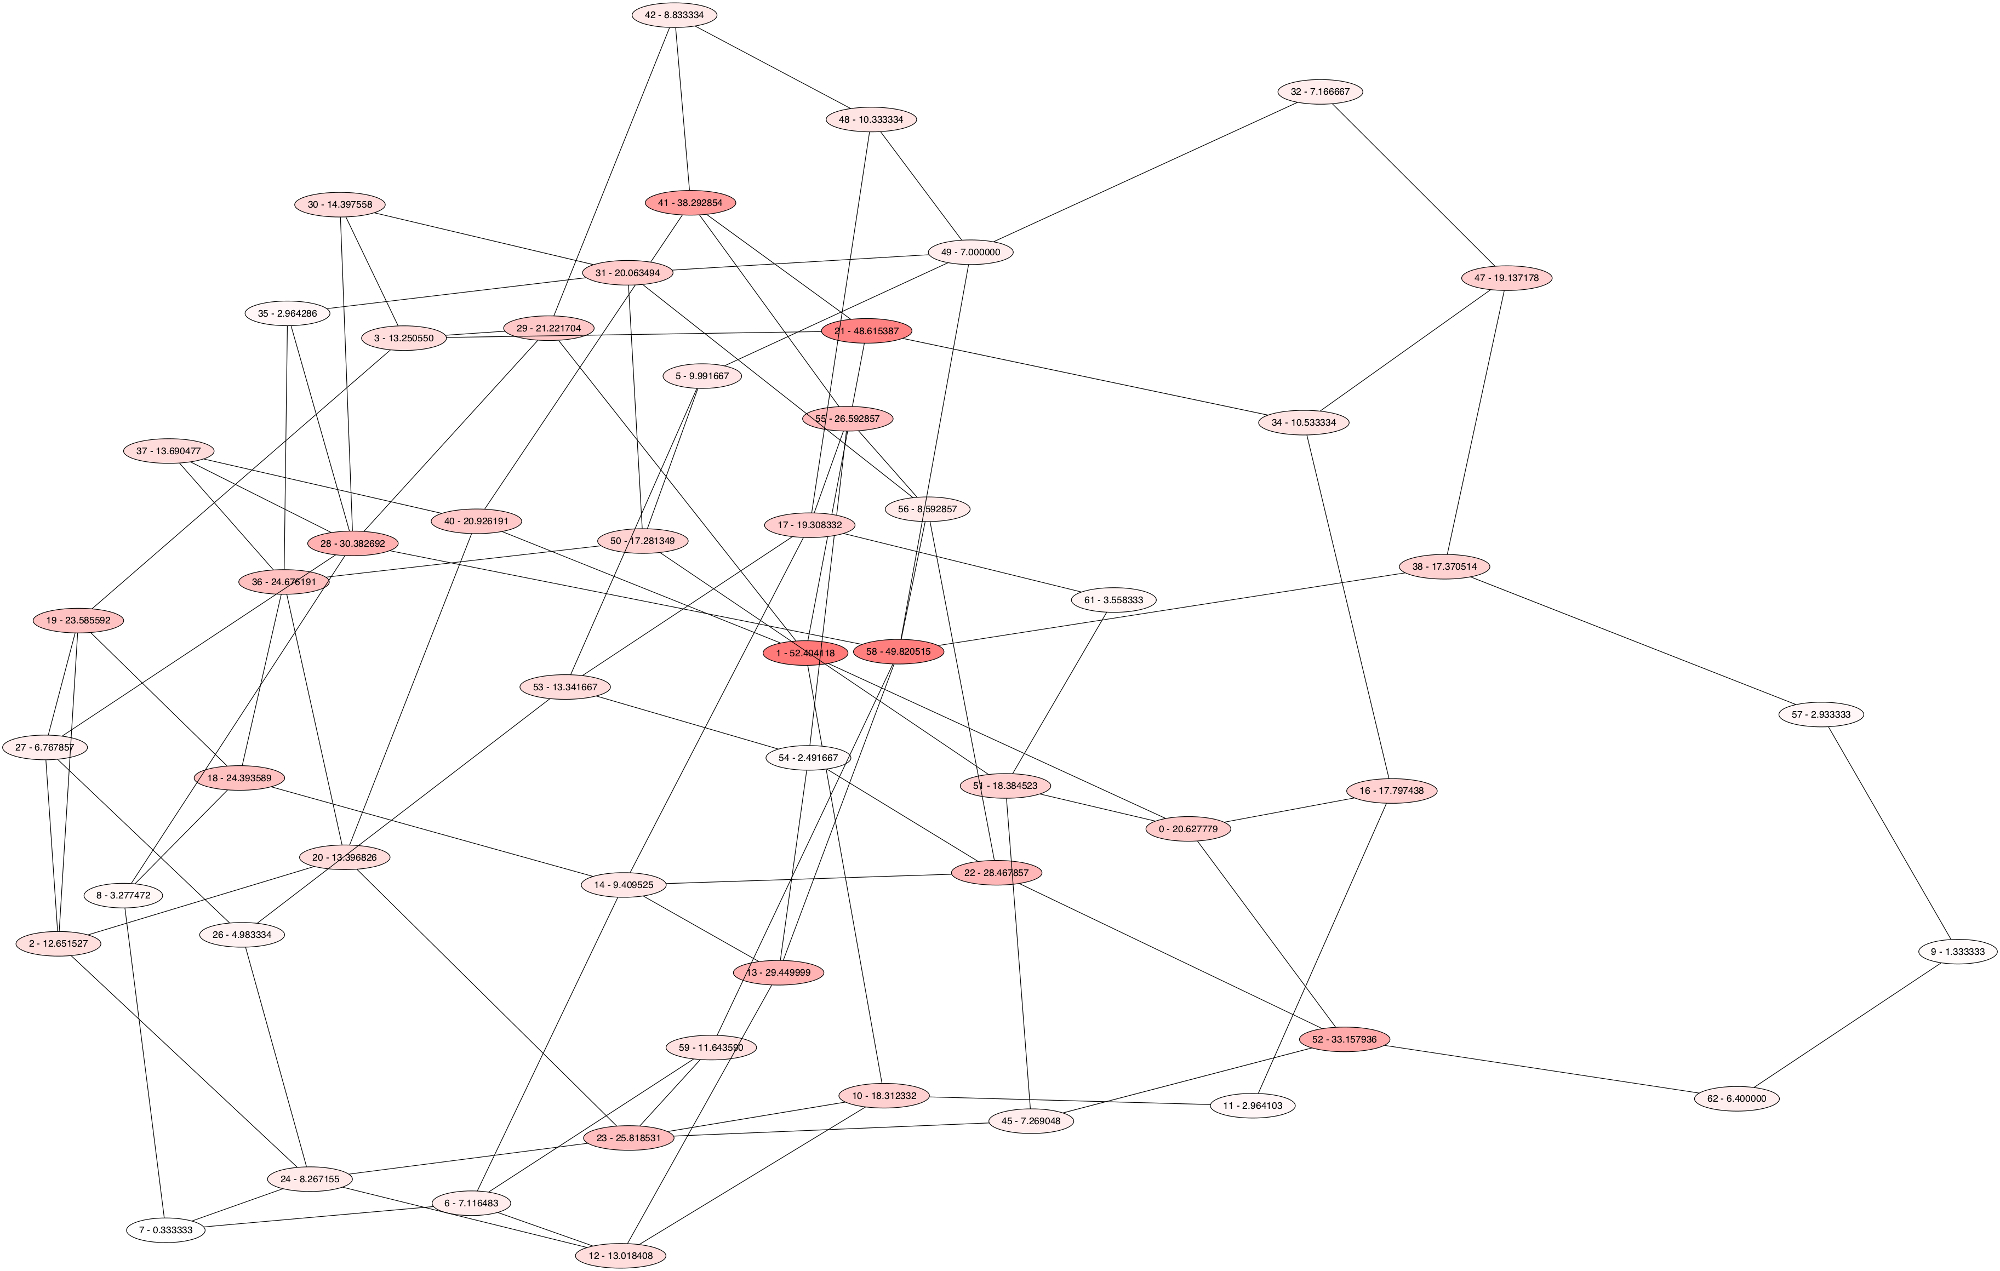
\includegraphics[width=0.9\textwidth]{figures/synthetic64_2}
%\caption{Synthetic with ~64 edges}
\end{center}
\begin{center}
\textit{Figure 1: Synthetic with ~64 edges}
\end{center}

\begin{center}
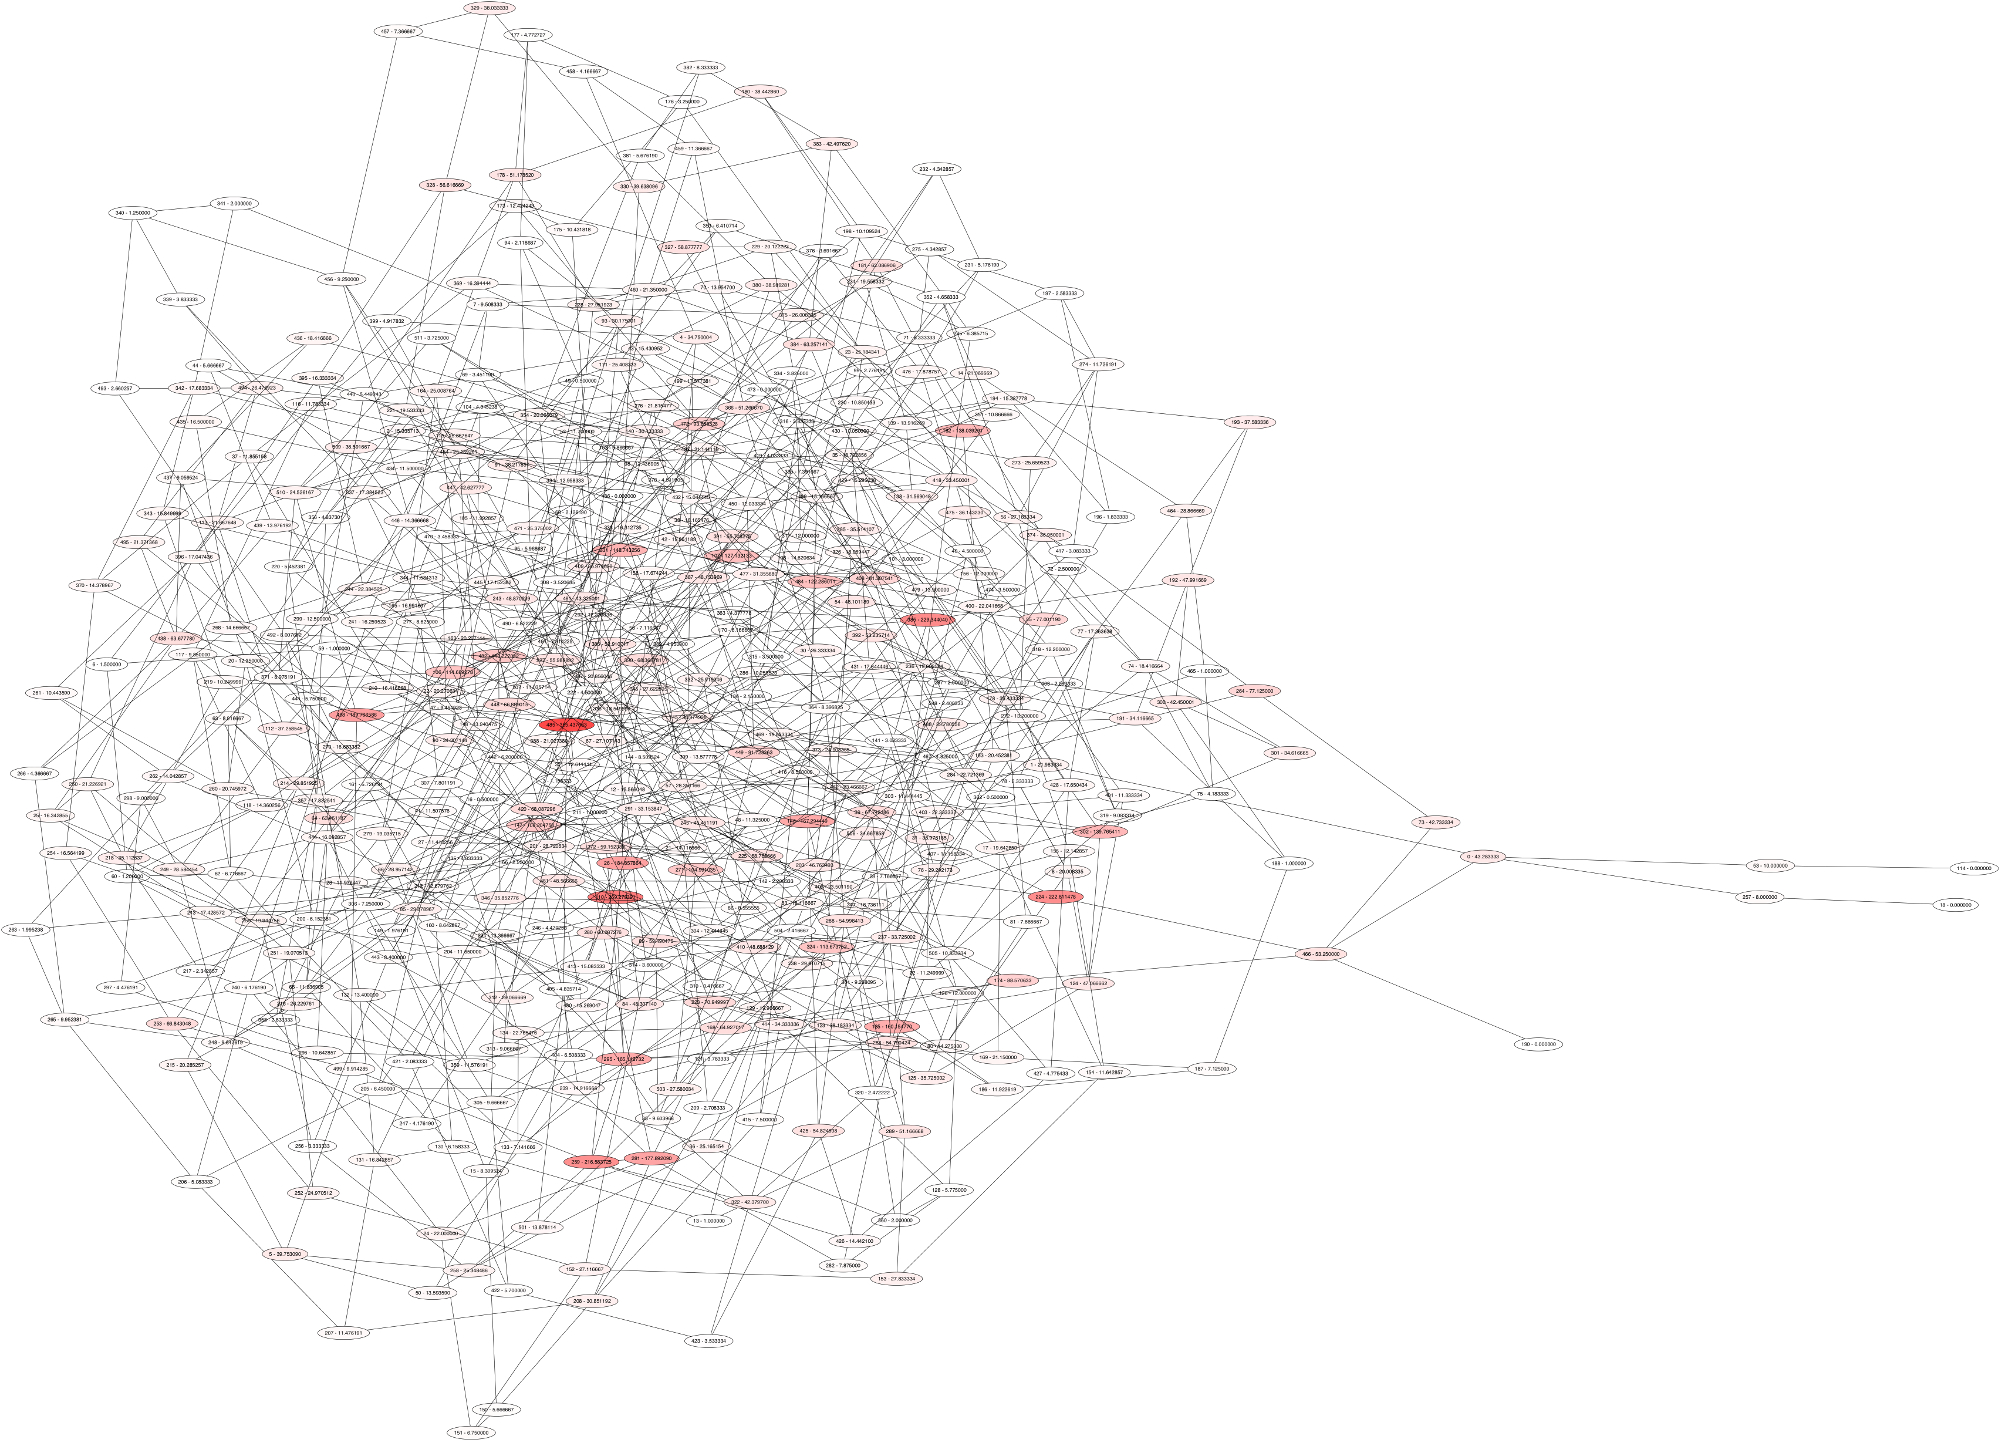
\includegraphics[width=0.9\textwidth]{figures/synthetic512_1}
%\caption{Synthetic with ~512 edges}
\end{center}
\begin{center}
\textit{Figure 2: Synthetic with ~512 edges}
\end{center}

The vertices with deeper reds have larger betweenness centrality metric values.

Once we were comfortable with our implementation, we found datasets used in a
Stanford paper by Leskovec and Mcauley \cite{leskovec2012learning}. We
downloaded this dataset and read it into memory. We ran this through our system
and generated the following Graphviz renderings:

\begin{center}
\includegraphics[width=0.9\textwidth]{figures/facebook}
%\caption{Facebook betweenness centrality calculation}
\end{center}
\begin{center}
\textit{Figure 3: Facebook betweenness centrality calculation}
\end{center}



%% ============================= Results ============================= %%
\section{Results} % 4. experiments and results
\label{sec:results}
%     * Challenges of rendering large graphs
%     * Challenges of validating centrality
%     * Graphs of strong and weak scalability.
%     * Graphs of centrality found

While the graphs we were able to generate were quite exciting, unfortunately
our implementation appears to have poor performance when scaling. This is most
likely due to memory contention from having the whole graph in shared memory.

\begin{center}
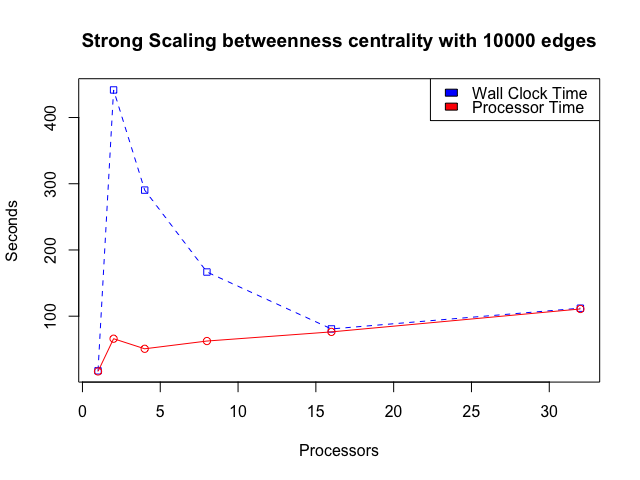
\includegraphics[width=0.8\textwidth]{figures/strong}
%\caption{Strong scaling for betweenness centrality on a synthetic graph with
%  10000 edges}
\end{center}
\begin{center}
\textit{Figure 4: Strong scaling for betweenness centrality on a synthetic
graph with 10000 edges}
\end{center}

\begin{center}
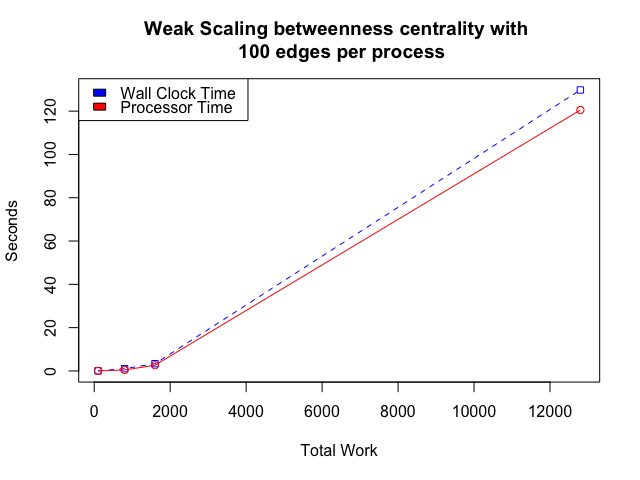
\includegraphics[width=0.8\textwidth]{figures/weak}
% \caption{Weak scaling for betweenness centrality on a synthetic graph with
%   100 edges per process}
\end{center}
\begin{center}
\textit{Figure 5: Weak scaling for betweenness centrality on a synthetic graph
with 100 edges per process}
\end{center}

This figure indicates that our implementation has very poor weak scaling. We
hypothesize that this stems from the use of the graph being used in shared
memory.



%% ============================= Conclusion ============================= %%
\section{Conclusion} % 5. conclusions and future directions
\label{sec:conclusion}

Our implementation of the Brandes' algorithm could be improved by distributing
the memory across the processors instead of using shared memory. With that said,
we achieved some interesting results in finding the vertices in a graph that
have high betweenness centrality.



%% ============================= Future Work ============================= %%
\section{Future Work}
\label{sec:future-work}
%     * We could continue working to improve the running time and finding more
%       graphs to run it on
%     * We used a shared memory model, it would be interesting to try and break
%       up the graph into a distributed memory model.

Looking forward, there are a number of improvements we could make. Our
scalability results showed poor performance, which is likely due to all of the
contention over the shared memory. If we had more time, we would like to
explore different options for distributing the graph across processors. In
addition we would like to try and find existing datasets that have already
performed betweenness centrality calculations so that we might validate our
metrics.



%% ============================= Bibliography ============================= %%
\newpage
\bibliographystyle{acm}
\bibliography{references}



\end{document}
